\chapter{Fractional Calculus}

The idea behind fractional operators started when L'Hôpital asked Leibniz whether an extension to integer-order derivatives could be done, i.e. $d^\alpha y/dx^\alpha$ when $\alpha\notin\mathbb{N}$. At the time, the idea did not captivate enough attention; nowadays, multiple physical applications have been proposed, mostly as generalization of known systems \cite{deng2012numerical}. 

On the other hand, fractional derivatives have multiple definitions, depending on the author that studied them; for example Euler, Fourier, Abel, Liouville, Riemann, Letnikov, Grünwald, Caputo, Miller, etc \cite{dalir2010applications}. In this book, the Caputo-type fractional derivatives will be used since, as we will discuss further in this work, they satisfy an important property to simulate physical systems.

Some applications of fractional calculus (from \cite{dalir2010applications}):
\begin{multicols}{2}
\begin{itemize}
    \item \textit{The tautochrone problem} (Abel's approach) \cite{kisela2008fractional}.
    \item \textit{Electric transmission lines} (Heaviside) \cite{heaviside1899theory}.
    \item \textit{Ultrasonic wave propagation in human cancellous bone} (Sebaa \textit{et al.}) \cite{sebaa2006application}.
    \item \textit{Modeling of speech signals using fractional calculus} (Assaleh \& Ahmad) \cite{assaleh2007modeling}.
    \item \textit{Modeling the cardiac tissue electrode interface using fractional calculus} (Magin \& Ovadia) \cite{magin2006modeling}.
    \item \textit{Application of fractional calculus to the sound waves propagation in rigid porous materials} (Fellah \& Depollier) \cite{fellah2002application}.
    \item \textit{Using fractional calculus for lateral and longitudinal control of autonomous vehicles} (Su\'arez \textit{et al.}) \cite{suarez2003using}.
    \item \textit{Application of fractional calculus in the theory of viscoelasticity} (Soczkiewicz) \cite{soczkiewicz2002application}.
    \item \textit{Fractional differentiation for edge detection} (Mathieu \textit{et al.}) \cite{mathieu2003fractional}.
    \item \textit{Wave propagation in viscoelastic horns using a fractional calculus rheology model} (Marguiles) \cite{margulies2003wave}.
    \item \textit{Application of fractional calculus to fluid mechanics} (Kulish \& Lage) \cite{kulish2002application}.
\end{itemize}
\end{multicols}

It is considered that fractional derivatives have some advantages and disadvantages
\begin{multicols}{2}
    \textbf{Advantages}
    \begin{itemize}
        \item Generalization of ordinary derivatives.
        \item Nonlocal operators $\longrightarrow$ Memory and heritage.
        \item More accuracy and robustness.
        \item Unexplored areas and applications.
    \end{itemize}
    \columnbreak
    \textbf{Disadvantages}
    \begin{itemize}
        \item There are multiple fractional derivatives definitions.
        \item The derivatives are not always in terms of elementary functions.
        \item Some definitions require strong conditions on the functions to differentiate.
    \end{itemize}
    \end{multicols}

\section{Preliminaries}
\subsection{Gamma Function}\label{subsec:gamma}
While treating fractional derivatives, the following definition will come in handy. The Gamma Function is defined by the improper integral

\begin{equation}
    \Gamma(z) = \int_0^\infty t^{z-1}e^{-t}dt\quad \mathrm{Re}(z)>0
\end{equation}

This function has some special properties: $\Gamma(z+1)=z\Gamma(z)$ and $\Gamma(1/2)=\sqrt{\pi}$. In figure \ref{fig:gamma}, the curve for the gamma function is shown.

\begin{figure}[H]
    \centering
    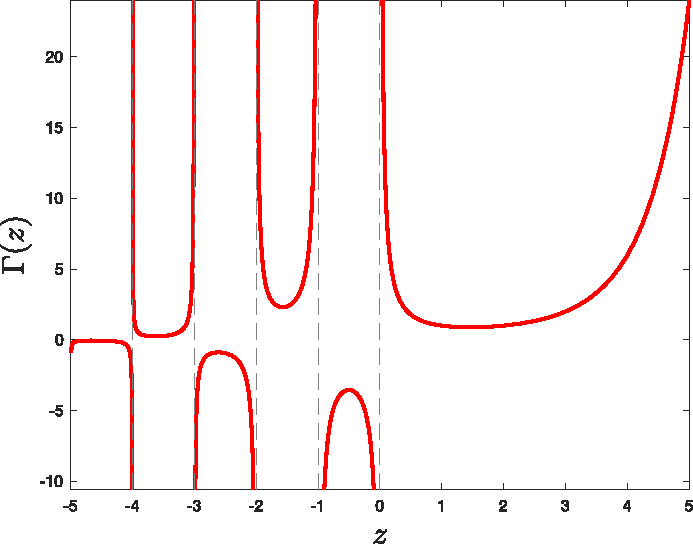
\includegraphics[scale=0.5]{files/gamma.pdf}
    \caption{The gamma function.}
    \label{fig:gamma}
\end{figure}

\subsection{Beta Function}
The Beta function is used for obtaining some important results in fractional calculus. This function is defined as

\begin{equation}
    B(z,w)=\int_0^1 t^{z-1}(1-t)^{w-1}dt\quad z,w>0
\end{equation}

The Beta function can be as well defined in terms of the Gamma function (section \ref{subsec:gamma})
\begin{equation}
    B(z,w)=\dfrac{\Gamma(z)\Gamma(w)}{\Gamma(z+w)}
\end{equation}
Note that $B(z,w)=B(w,z)$.

\subsection{Mittag-Leffler Function}
The Mittag-Leffler function is a special-complex function defined as
\begin{equation}
    E_{\alpha,\beta}(z)=\sum_{k=0}^{\infty}\dfrac{z^k}{\Gamma(\alpha k +\beta)} \quad z\in\mathbb{C}
\end{equation}

Where $\alpha,\,\beta\in\mathbb{R}$ and $\Gamma(\cdot)$ is the gamma function. 

\begin{figure}[H]
    \centering
    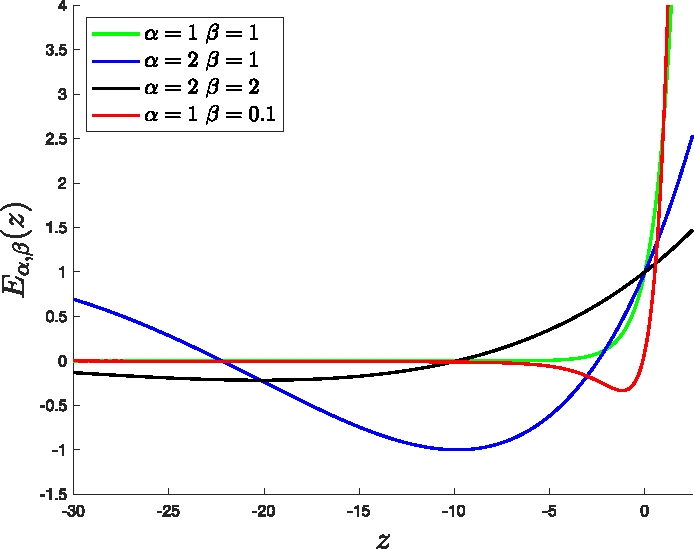
\includegraphics[scale=0.5]{files/mittag.pdf}
    \caption{Mittag-Leffler functions for some $\alpha$ and $\beta$.}
    \label{fig:mittag}
\end{figure}
